% ~8 pages
\subsection{Orthogonal Frequency Division Multiplexing}

Orthogonal Frequency Division Multiplexing (OFDM) has become the dominant waveform technology in modern wireless communication systems due to its high spectral efficiency and implementation simplicity. OFDM has been adopted in numerous communication standards, including LTE, 5G NR, Wi-Fi, and digital broadcasting systems. Before discussing the limitations of OFDM in high-mobility environments and the motivation for OTFS modulation, it is necessary to understand its fundamental operating principles.

\subsubsection{Principles of OFDM}

Orthogonal Frequency Division Multiplexing (OFDM) is a multicarrier transmission technique that divides a high-rate data stream into multiple parallel low-rate data streams. These streams are transmitted simultaneously over a set of orthogonal subcarriers, thereby reducing the symbol rate associated with each subcarrier and improving robustness against frequency-selective fading.

Unlike conventional Frequency Division Multiplexing (FDM), where adjacent subcarriers must be separated by guard bands to prevent interference, OFDM exploits the orthogonality between subcarriers to allow significant spectral overlap. As a result, OFDM achieves high spectral efficiency while maintaining the ability to separate individual subcarriers at the receiver.

The baseband OFDM signal can be expressed as

\begin{equation}
s(t)=\sum_{k=0}^{N-1} X_k e^{j2\pi k\Delta f t},
\quad 0 \le t < T
\end{equation}

where \(X_k\) denotes the complex symbol transmitted on the \(k\)-th subcarrier, \(N\) is the total number of subcarriers, and \(\Delta f\) represents the subcarrier spacing.

The key feature of OFDM is the orthogonality among subcarriers. Two subcarriers are orthogonal when

\begin{equation}
\int_{0}^{T}
e^{j2\pi n\Delta f t}
e^{-j2\pi m\Delta f t}
dt
=
0,
\quad n \neq m
\end{equation}

which is satisfied when the subcarrier spacing is chosen as

\begin{equation}
\Delta f = \frac{1}{T}
\end{equation}

where \(T\) denotes the OFDM symbol duration.

\begin{figure}[H]
    \centering
    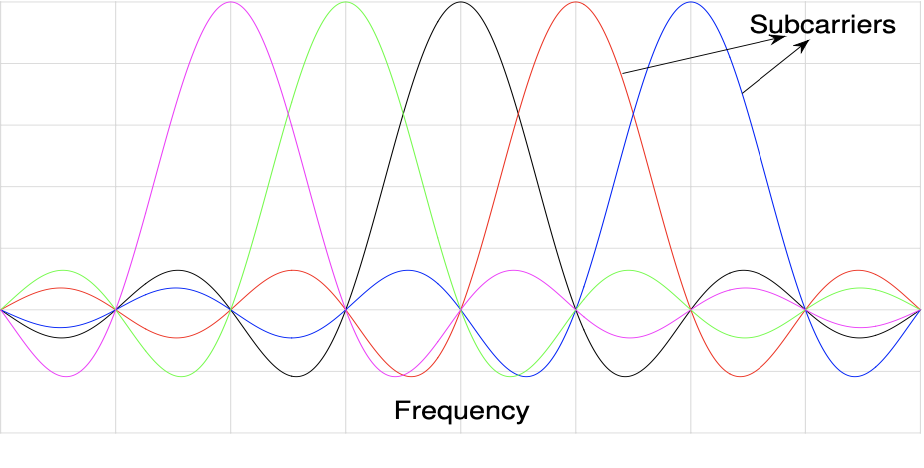
\includegraphics[width=1\textwidth]{Images/Chapter2/ofdmsubcarrier.png}
    \caption[Orthogonality among OFDM subcarriers.]{Orthogonality among OFDM subcarriers~\protect\cite{ScienceDirectICI}.}
    \label{fig:ofdm_orthogonality}
\end{figure}

As illustrated in Fig.~\ref{fig:ofdm_orthogonality}, the spectrum of each subcarrier exhibits a sinc-shaped response. Although adjacent subcarriers overlap significantly in the frequency domain, the peak of one subcarrier coincides with the null points of all other subcarriers. Consequently, mutual interference is avoided and the transmitted symbols can be recovered independently.

A major advantage of OFDM is its efficient implementation using the Inverse Fast Fourier Transform (IFFT) and Fast Fourier Transform (FFT). At the transmitter, information symbols are mapped onto frequency-domain subcarriers and transformed into the time domain using an IFFT operation. At the receiver, an FFT operation is applied to recover the transmitted symbols from the received waveform.

\begin{figure}[H]
    \centering
    \resizebox{0.95\textwidth}{!}{
    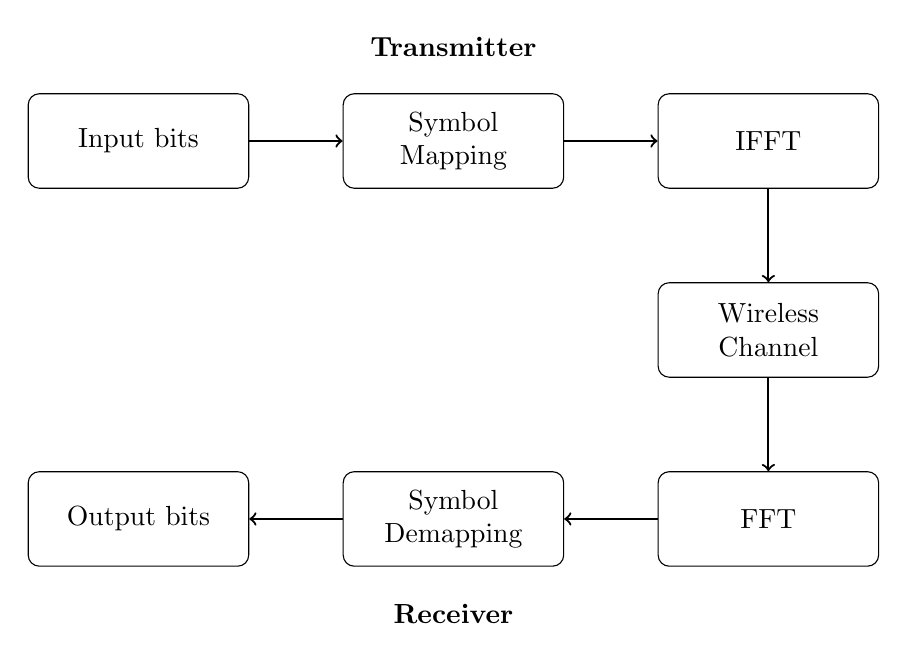
\begin{tikzpicture}[
        block/.style={
            draw,
            rounded corners,
            minimum width=2.8cm,
            minimum height=1.2cm,
            align=center,
            font=\normalsize
        },
        arrow/.style={->, thick}
    ]

    % =========================
    % Transmitter
    % =========================
    \node[block] (in)   at (0,2.4) {Input bits};
    \node[block] (map)  at (4.0,2.4) {Symbol\\Mapping};
    \node[block] (ifft) at (8.0,2.4) {IFFT};

    \draw[arrow] (in) -- (map);
    \draw[arrow] (map) -- (ifft);

    \node[font=\bfseries] at (4.0,3.6) {Transmitter};

    % =========================
    % Channel
    % =========================
    \node[block] (channel) at (8.0,0) {Wireless\\Channel};
    \draw[arrow] (ifft) -- (channel);

    % =========================
    % Receiver
    % =========================
    \node[block] (fft)   at (8.0,-2.4) {FFT};
    \node[block] (demap) at (4.0,-2.4) {Symbol\\Demapping};
    \node[block] (out)   at (0,-2.4) {Output bits};

    \draw[arrow] (channel) -- (fft);
    \draw[arrow] (fft) -- (demap);
    \draw[arrow] (demap) -- (out);

    \node[font=\bfseries] at (4.0,-3.6) {Receiver};

    \end{tikzpicture}
    }
    \caption{Basic principle of OFDM transmission using IFFT and FFT operations.}
    \label{fig:ofdm_basic_principle}
\end{figure}

By converting a broadband frequency-selective channel into multiple narrowband subchannels, OFDM significantly simplifies receiver design and equalization. This property has contributed to its widespread adoption in modern wireless communication systems. However, despite these advantages, OFDM experiences considerable performance degradation in rapidly time-varying channels, particularly under high Doppler conditions. These limitations are discussed in the following subsections.


\subsubsection{OFDM Transceiver Structure}

The practical implementation of OFDM systems is based on digital signal processing techniques that efficiently generate and recover orthogonal subcarriers using IFFT and FFT operations. Instead of using a large number of separate oscillators and modulators for different subcarriers, OFDM generates all subcarriers jointly through an inverse Fourier transform. This significantly reduces implementation complexity while maintaining high spectral efficiency.

A typical OFDM transceiver consists of a transmitter, a wireless propagation channel, and a receiver. At the transmitter, the input binary data stream is first converted into parallel data streams. These bits are then mapped into complex modulation symbols using modulation schemes such as BPSK, QPSK, or QAM. The resulting symbols are assigned to different frequency-domain subcarriers.

To generate the time-domain OFDM waveform, an \(N\)-point Inverse Fast Fourier Transform (IFFT) is applied to the frequency-domain symbols. The IFFT converts the parallel subcarrier symbols into a discrete-time OFDM signal while preserving the orthogonality among subcarriers. The transmitted OFDM symbol can be expressed as

\begin{equation}
x[n]
=
\frac{1}{\sqrt{N}}
\sum_{k=0}^{N-1}
X[k]
e^{j\frac{2\pi kn}{N}},
\quad n=0,1,\ldots,N-1,
\end{equation}

where \(X[k]\) denotes the modulation symbol transmitted on the \(k\)-th subcarrier and \(N\) represents the total number of subcarriers.

In practical OFDM systems, a cyclic prefix (CP) is often appended to each OFDM symbol before transmission. The CP is formed by copying the last portion of the OFDM symbol and inserting it at the beginning of the symbol interval. This operation helps mitigate inter-symbol interference (ISI) caused by multipath propagation and allows the linear convolution of the channel to be treated approximately as circular convolution. As a result, frequency-domain equalization at the receiver becomes much simpler.

\begin{figure}[H]
    \centering
    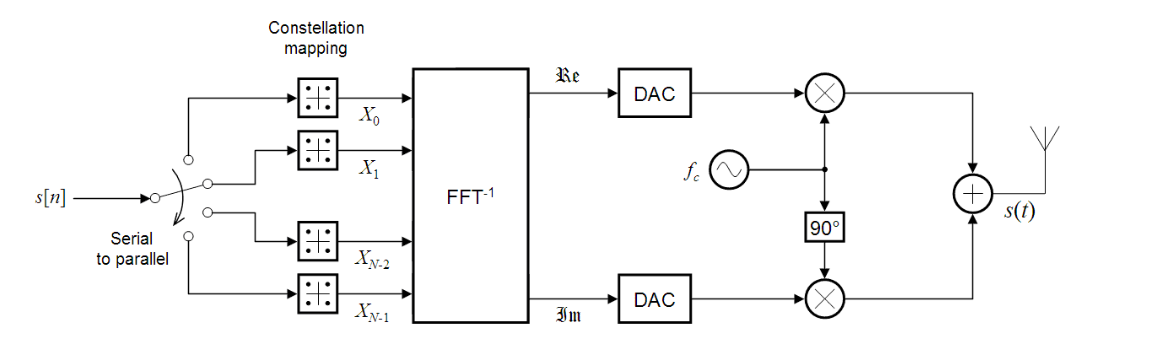
\includegraphics[width=0.92\textwidth]{Images/Chapter2/ofdmtx.png}
    \caption[OFDM transmitter structure.]{OFDM transmitter structure~\protect\cite{Hong2019OTFSTutorial}.}
    \label{fig:ofdm_tx}
\end{figure}

\begin{figure}[H]
    \centering
    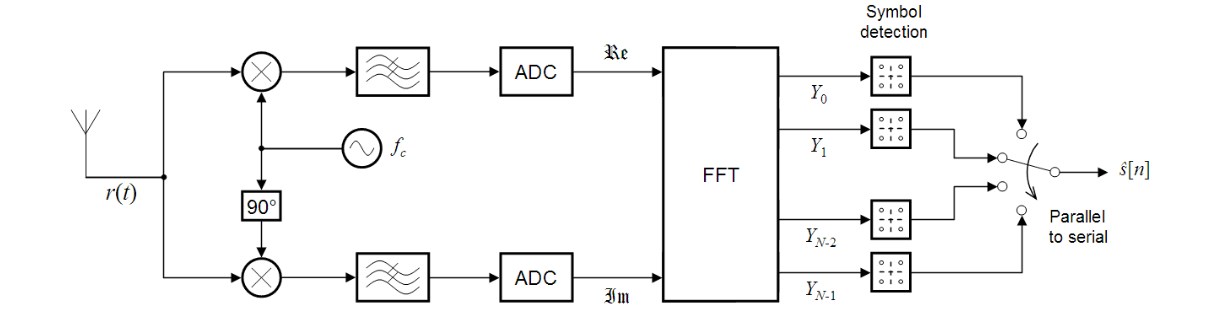
\includegraphics[width=0.92\textwidth]{Images/Chapter2/ofdmrx.png}
    \caption[OFDM receiver structure.]{OFDM receiver structure~\protect\cite{Hong2019OTFSTutorial}.}
    \label{fig:ofdm_rx}
\end{figure}



As illustrated in Fig.~\ref{fig:ofdm_tx}, the transmitter performs serial-to-parallel conversion, constellation mapping, IFFT processing, digital-to-analog conversion, and carrier modulation before radiating the signal through the antenna. The IFFT block is the key baseband processing stage because it converts frequency-domain subcarrier symbols into a time-domain waveform suitable for transmission.

After propagating through the wireless channel, the received signal is affected by multipath fading, Doppler shifts, and additive noise. At the receiver, the signal is first downconverted from the carrier frequency, filtered, and converted back into digital samples. The FFT operation is then applied to transform the received time-domain signal back into the frequency domain. Symbol detection and parallel-to-serial conversion are finally performed to recover the estimated transmitted bit sequence.

Under the assumption that the channel remains approximately constant during one OFDM symbol interval and that the CP is sufficiently long, the received symbol on the \(k\)-th subcarrier can be represented as

\begin{equation}
Y[k]
=
H[k]X[k]
+
W[k],
\end{equation}

where \(Y[k]\) is the received symbol on the \(k\)-th subcarrier, \(H[k]\) denotes the channel frequency response, \(X[k]\) is the transmitted symbol, and \(W[k]\) represents the noise component.

Because each OFDM subcarrier experiences an approximately flat channel response, equalization can be performed independently for each subcarrier. This one-tap frequency-domain equalization greatly reduces receiver complexity compared with single-carrier systems operating over frequency-selective channels.

The use of FFT-based processing and simple per-subcarrier equalization is one of the main reasons for the widespread adoption of OFDM in modern wireless communication systems. However, these advantages rely on the assumption that the channel is nearly time-invariant within each OFDM symbol. In high-mobility environments, Doppler spread causes rapid channel variation and may destroy the orthogonality among subcarriers, resulting in inter-carrier interference and degraded system performance.


\subsubsection{Advantages of OFDM}

OFDM has been widely adopted in modern wireless communication systems because it provides an efficient solution for transmission over frequency-selective fading channels. By dividing a wideband channel into a large number of narrowband orthogonal subchannels, OFDM simplifies the equalization problem and enables reliable high-data-rate transmission.

One of the most important advantages of OFDM is its robustness against multipath propagation. In a single-carrier system, multipath delay spread may cause severe inter-symbol interference because delayed replicas of previous symbols overlap with the current symbol. In OFDM, the symbol duration on each subcarrier is increased by transmitting data in parallel over many subcarriers. As a result, the relative impact of delay spread is reduced.

Another major advantage is the use of the cyclic prefix. When the cyclic prefix length is longer than the maximum delay spread of the channel, the linear convolution between the transmitted signal and the multipath channel can be transformed into circular convolution. This allows the frequency-selective channel to be represented as a set of parallel flat-fading subchannels after the FFT operation at the receiver.

Under ideal synchronization and sufficiently slow channel variation, the received signal on each subcarrier follows the one-tap input-output relation introduced in the previous subsection. Since the transmitted symbols are separated in the frequency domain, each subcarrier can be equalized independently using a one-tap equalizer.

The estimated transmitted symbol can therefore be obtained as

\begin{equation}
\hat{X}[k]=\frac{Y[k]}{H[k]},
\end{equation}

where \(H[k]\) is the channel frequency response on the \(k\)-th subcarrier.

This one-tap frequency-domain equalization is one of the key reasons for the practical success of OFDM. Compared with time-domain equalization in wideband single-carrier systems, OFDM significantly reduces receiver complexity.

\begin{figure}[H]
    \centering
    \resizebox{0.95\textwidth}{!}{
    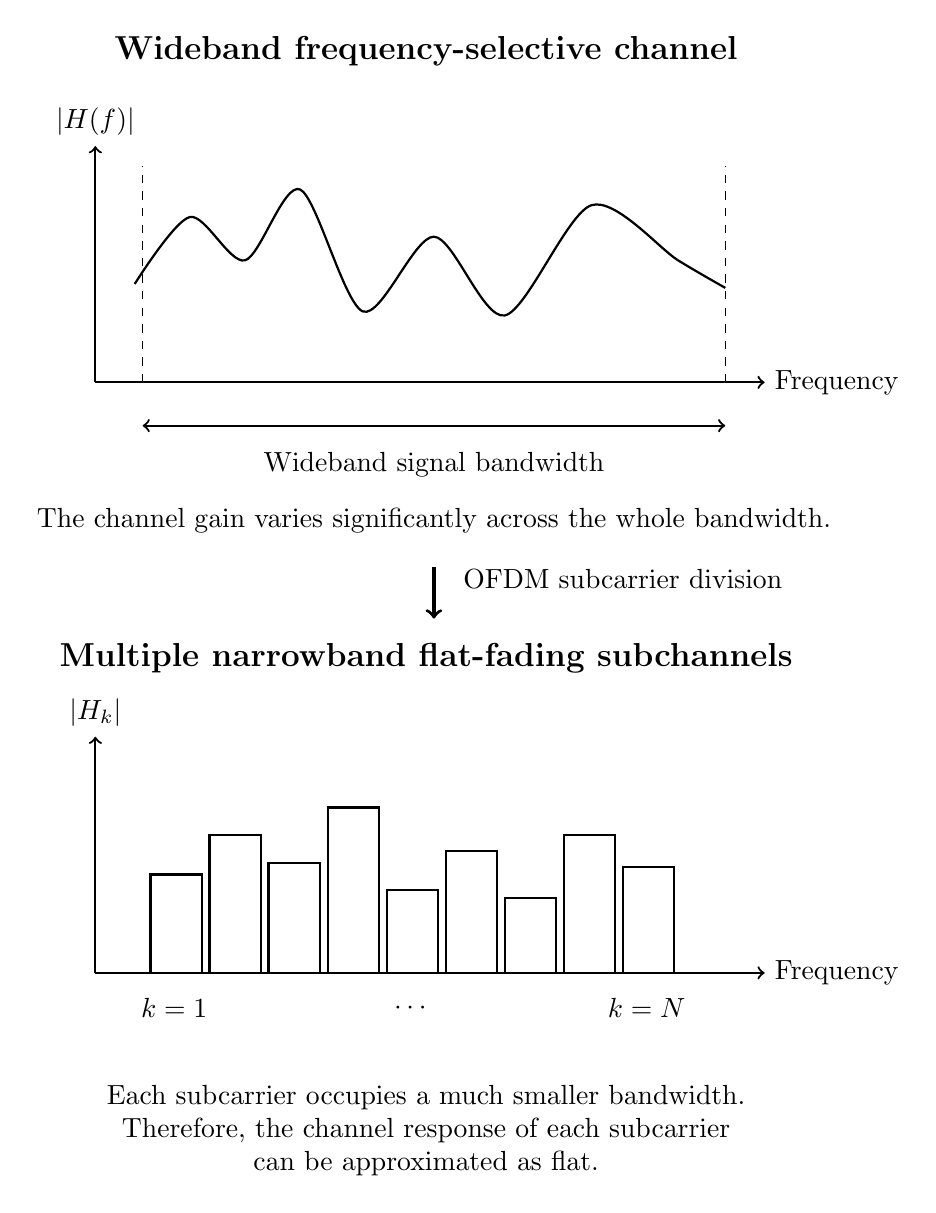
\begin{tikzpicture}[
        every node/.style={font=\normalsize},
        axis/.style={->, thick},
        thickline/.style={thick}
    ]

    % =====================================================
    % Top: Wideband frequency-selective channel
    % =====================================================
    \node[font=\bfseries\large] at (4.2,4.2)
    {Wideband frequency-selective channel};

    \draw[axis] (0,0) -- (8.5,0) node[right] {Frequency};
    \draw[axis] (0,0) -- (0,3.0) node[above] {$|H(f)|$};

    % Frequency-selective response
    \draw[thickline]
        plot[smooth] coordinates {
        (0.5,1.25)
        (1.2,2.10)
        (1.9,1.55)
        (2.6,2.45)
        (3.4,0.90)
        (4.3,1.85)
        (5.2,0.85)
        (6.3,2.25)
        (7.4,1.55)
        (8.0,1.20)
        };

    % Bandwidth marks
    \draw[dashed] (0.6,0) -- (0.6,2.75);
    \draw[dashed] (8.0,0) -- (8.0,2.75);

    \draw[<->, thick] (0.6,-0.55) -- (8.0,-0.55);
    \node at (4.3,-1.05) {Wideband signal bandwidth};

    % Explanation label
    \node[align=center] at (4.3,-1.75)
    {The channel gain varies significantly across the whole bandwidth.};

    % =====================================================
    % Down arrow
    % =====================================================
    \draw[->, very thick] (4.3,-2.35) -- (4.3,-3.0);
    \node[right] at (4.55,-2.5) {OFDM subcarrier division};

    % =====================================================
    % Bottom: Narrowband subchannels
    % =====================================================
    \begin{scope}[yshift=-7.5cm]

    \node[font=\bfseries\large] at (4.2,4.0)
    {Multiple narrowband flat-fading subchannels};

    \draw[axis] (0,0) -- (8.5,0) node[right] {Frequency};
    \draw[axis] (0,0) -- (0,3.0) node[above] {$|H_k|$};

    % Draw narrow flat subchannels
    \draw[thick] (0.7,0) rectangle (1.35,1.25);
    \draw[thick] (1.45,0) rectangle (2.10,1.75);
    \draw[thick] (2.20,0) rectangle (2.85,1.40);
    \draw[thick] (2.95,0) rectangle (3.60,2.10);
    \draw[thick] (3.70,0) rectangle (4.35,1.05);
    \draw[thick] (4.45,0) rectangle (5.10,1.55);
    \draw[thick] (5.20,0) rectangle (5.85,0.95);
    \draw[thick] (5.95,0) rectangle (6.60,1.75);
    \draw[thick] (6.70,0) rectangle (7.35,1.35);

    % Labels
    \node at (1.0,-0.45) {$k=1$};
    \node at (4.0,-0.45) {$\cdots$};
    \node at (7.0,-0.45) {$k=N$};

    \node[align=center] at (4.2,-2)
    {Each subcarrier occupies a much smaller bandwidth.\\
    Therefore, the channel response of each subcarrier\\
    can be approximated as flat.};

    \end{scope}

    \end{tikzpicture}
    }

    \caption{Conversion of a frequency-selective wideband channel into multiple narrowband flat-fading subchannels in OFDM.}
    \label{fig:ofdm_parallel_subchannels}
\end{figure}


OFDM also provides high spectral efficiency due to the orthogonality among subcarriers. Unlike conventional frequency division multiplexing, which requires guard bands between adjacent carriers, OFDM allows subcarrier spectra to overlap while still avoiding mutual interference under ideal conditions. This property makes OFDM particularly suitable for bandwidth-limited wireless communication systems.

The main advantages of OFDM are summarized in Table~\ref{tab:ofdm_advantages}.

\begin{table}[H]
\centering
\caption{Main advantages of OFDM systems.}
\label{tab:ofdm_advantages}

\begin{tabular}{|p{4cm}|p{8cm}|}
\hline
\textbf{Advantage} &
\textbf{Description} \\
\hline

High spectral efficiency &
Overlapping orthogonal subcarriers reduce the need for guard bands. \\
\hline

Robustness to multipath &
Longer symbol duration and cyclic prefix reduce the effect of delay spread. \\
\hline

Simple equalization &
Frequency-selective channels are transformed into parallel flat-fading subchannels. \\
\hline

FFT-based implementation &
IFFT and FFT operations enable efficient digital implementation. \\
\hline

Flexible resource allocation &
Subcarriers can be assigned adaptively according to channel conditions and user requirements. \\
\hline

\end{tabular}

\end{table}

Despite these advantages, OFDM relies heavily on the preservation of subcarrier orthogonality. This requirement becomes difficult to satisfy in rapidly time-varying wireless channels, especially when the receiver operates under high mobility. The limitations of OFDM under such conditions are discussed in the following subsection.

\subsubsection{Limitations of OFDM in High-Mobility Environments}

Although OFDM is highly effective in combating frequency-selective fading, its performance can degrade significantly in high-mobility environments. The main reason is that OFDM assumes the wireless channel remains approximately constant during one OFDM symbol duration. When this assumption is violated, the orthogonality among subcarriers is destroyed.

In high-mobility scenarios, relative motion between the transmitter, receiver, and scatterers introduces Doppler shifts. These Doppler shifts cause the channel response to vary within an OFDM symbol interval. Consequently, the received signal is no longer affected only by the channel gain on its own subcarrier, but also by leakage from neighboring subcarriers. This phenomenon is known as inter-carrier interference (ICI).

Under ideal conditions, the received signal on the \(k\)-th subcarrier is represented by

\begin{equation}
Y[k]=H[k]X[k]+W[k].
\end{equation}

However, in the presence of Doppler-induced channel variation, the received signal becomes

\begin{equation}
Y[k]=H[k]X[k]+\sum_{\substack{m=0 \\ m\neq k}}^{N-1} I[k,m]X[m]+W[k],
\end{equation}

where \(I[k,m]\) represents the interference contribution from the \(m\)-th subcarrier to the \(k\)-th subcarrier. The second term in the equation represents inter-carrier interference caused by the loss of orthogonality.

\begin{figure}[H]
    \centering
    
\includegraphics[width=1\textwidth]{Images/Chapter2/ici.png}
    \caption[Inter-carrier interference in OFDM caused by Doppler-induced loss of subcarrier orthogonality.]{Inter-carrier interference in OFDM caused by Doppler-induced loss of subcarrier orthogonality~\protect\cite{Hong2019OTFSTutorial}.}
    \label{fig:ofdm_ici}
\end{figure}

As illustrated in Fig.~\ref{fig:ofdm_ici}, Doppler shifts disturb the frequency-domain alignment of OFDM subcarriers. The null points of one subcarrier no longer coincide with the peaks of other subcarriers, causing interference among subcarriers. This effect becomes more severe as the Doppler spread increases.

Another limitation of OFDM is that the performance of the system is strongly affected by the weakest subcarriers. In a frequency-selective fading channel, some subcarriers may experience deep fading while others maintain strong channel gains. Although coding and interleaving can mitigate this problem to some extent, the overall reliability of the system may still be limited by poorly conditioned subchannels.

Furthermore, the one-tap equalization structure of OFDM is only effective when the channel matrix remains nearly diagonal in the frequency domain. In high-Doppler conditions, the channel matrix loses this diagonal structure due to ICI. Equalization therefore becomes more complex, and the simplicity that makes OFDM attractive is partially lost.

\begin{table}[H]
\centering
\caption{Main limitations of OFDM in high-mobility environments.}
\label{tab:ofdm_limitations}

\begin{tabular}{|p{4cm}|p{8cm}|}
\hline
\textbf{Limitation} &
\textbf{Impact} \\
\hline

Sensitivity to Doppler spread &
Doppler shifts destroy subcarrier orthogonality and introduce ICI. \\
\hline

Channel time variation &
The channel may change within one OFDM symbol, violating the quasi-static channel assumption. \\
\hline

Deep fading on subcarriers &
Some subcarriers may experience severe attenuation, reducing reliability. \\
\hline

Increased equalization complexity &
The channel matrix is no longer diagonal under severe Doppler conditions. \\
\hline

Performance degradation in high mobility &
BER increases significantly in vehicular, high-speed railway, UAV, and satellite communication scenarios. \\
\hline

\end{tabular}

\end{table}

These limitations motivate the search for alternative waveform designs that can better handle doubly selective channels. Instead of representing information symbols only in the time-frequency domain, OTFS modulation introduces a delay-Doppler domain representation where the channel can be described more compactly and more stably under high mobility. Before introducing OTFS in detail, the next section reviews the delay-Doppler domain representation of wireless channels.
